\section{BrowsableStoreAnalytics}\label{browsablestoreanalytics}

This is a project that demonstrates how virtual reality may be used to
gather better analytics from users when evaluating environments. Many
companies maintain large spaces in which to prototype store layouts and
designs. Constructing spaces in virtual reality is cheaper and allows a
company to gather more data from testing than a simple survey.

\section{First Time Setup}\label{first-time-setup}

\subsection{Setting Up Prerequisites}\label{setting-up-prerequisites}

This section taken from
\url{https://calben.gitbooks.io/unreal-engine-as-a-research-framework/content/chapter1.html}

\subsubsection{Unreal Engine}\label{unreal-engine}

This may come as some surprise, but start by installing Unreal Engine
(UE4). There are good instructions on how to do this here:
\url{https://docs.unrealengine.com/latest/INT/GettingStarted/Installation/}

\subsubsection{Visual Studio 2017}\label{visual-studio-2017}

As of date of publication, Visual Studio (VS) 2017 is the latest version
of VS, so you can pick this up here:
\url{https://www.visualstudio.com/downloads/}. When you do the install,
make sure to go to the ``Games'' tab and install the C++ features
available there (TODO go back and find the exact set of features that
need to be selected to ensure everything will work during the monthly
reset)

\subsubsection{Docker Toolbox for
Windows}\label{docker-toolbox-for-windows}

We will use the Docker Toolbox to host our TICK stack. You may pick up
the Docker Tools here:
\url{https://www.docker.com/products/docker-toolbox}. When installing,
choose to install Kitematic. If you have HyperV enabled on your machine,
you can use the HyperV implementation. If you don't have HyperV running
(or have the Home version of Windows), then you're going to need
Virtualbox.

\subsection{Setting Up the TICK Stack}\label{setting-up-the-tick-stack}

This section taken from
\url{https://calben.gitbooks.io/unreal-engine-as-a-research-framework/content/setting-up-the-tick-stack.html}

We're going to set up the TICK stack using Docker. If you wanted to
install it on a remote server, you could follow the documentation here:
\url{https://docs.influxdata.com/chronograf/v1.3/introduction/getting-started/}

\subsubsection{What Is TICK?}\label{what-is-tick}

TICK stands for Telegraf, InfluxDb, Chronograf, and Kapacitor. For
convenience, I am going to quote descriptions of the TICK stack here:

\paragraph{Telegraf}\label{telegraf}

\begin{quote}
\href{https://www.influxdata.com/time-series-platform/telegraf/}{Telegraf}
is a plugin-driven server agent for collecting and reporting metrics.
Telegraf has plugins or
\href{https://www.influxdata.com/products/integrations/}{integrations}
to source a variety of metrics directly from the system it's running on,
pull metrics from third party APIs, or even listen for metrics via a
StatsD and Kafka consumer services. It also has output plugins to send
metrics to a variety of other datastores, services, and message queues,
including InfluxDB, Graphite, OpenTSDB, Datadog, Librato, Kafka, MQTT,
NSQ, and many others.
\end{quote}

\paragraph{InfluxDB}\label{influxdb}

\begin{quote}
\href{https://www.influxdata.com/time-series-platform/influxdb/}{InfluxDB}
is a \href{https://www.influxdata.com/time-series-database/}{Time Series
Database} built from the ground up to handle high write \& query loads.
InfluxDB is a custom high performance datastore written specifically for
timestamped data, including DevOps monitoring, application metrics, IoT
sensor data, \& real-time analytics. Conserve space on your machine by
configuring InfluxDB to keep data for a defined length of time,
automatically expiring \& deleting any unwanted data from the system.
InfluxDB also offers a SQL-like query language for interacting with
data.
\end{quote}

\paragraph{Chronograf}\label{chronograf}

\begin{quote}
\href{https://www.influxdata.com/time-series-platform/chronograf/}{Chronograf}
is the administrative user interface and visualization engine of the
platform. It makes the monitoring and alerting for your infrastructure
easy to setup and maintain. It is simple to use and includes templates
and libraries to allow you to rapidly build dashboards with real-time
visualizations of your data and easily create alerting and automation
rules.
\end{quote}

\paragraph{Kapacitor}\label{kapacitor}

\begin{quote}
Kapacitor is a native data processing engine. It can process both stream
and batch data from InfluxDB. Kapacitor lets you plug in your own custom
logic or user-defined functions to process alerts with dynamic
thresholds, match metrics for patterns, compute statistical anomalies,
and perform specific actions based on these alerts like dynamic load
rebalancing. Kapacitor integrates with HipChat, OpsGenie, Alerta, Sensu,
PagerDuty, Slack, and
\href{https://www.influxdata.com/products/integrations/}{more}.
\end{quote}

\subsubsection{Running the Setup}\label{running-the-setup}

Assuming we're going the Docker route, you need to do the following:

\begin{enumerate}
\def\labelenumi{\arabic{enumi}.}
\tightlist
\item
  Start up Kitematic. You will be asked to use virtualbox if the program
  can't find a ``native'' setup (HyperV). Use VirtualBox if no native
  setup is fine, otherwise you shouldn't see a message.
\item
  You will be presented with a message that says ``Starting a Docker
  VM.'' This is creating a virtual machine for you called
  \texttt{default} that will be used to host your Docker containers.
\item
  After this runs, you're ready to set up your Docker containers! You
  will be asked to log in to Docker Hub. I recommend you make an account
  or log in, but if you'd rather not there's a ``Skip For Now'' hidden
  in the bottom right corner.
\item
  You should now be at the home menu for Kitematic. We're going to use
  the Docker command line to enter the below instructions:
\end{enumerate}

\begin{verbatim}
docker network create influxdb
docker run -d -p 8086:8086 --name=influxdb \
        --net=influxdb library/influxdb
docker run -d -p 9092:9092 --name=kapacitor \
        -v kapacitor:/var/lib/kapacitor --net=influxdb \ 
        -e KAPACITOR_INFLUXDB_0_URLS_0=http://influxdb:8086 library/kapacitor
docker run -d -p 8888:8888 --name=chronograf \
        --net=influxdb library/chronograf \
        --influxdb-url=http://influxdb:8086
\end{verbatim}

If you want to know what we just did, here is a version of the commands
to run with comments:

\begin{verbatim}
# create a new network called influxdb.
# docker containers connected to the image can access it with http://influxdb:<portname>
docker network create influxdb

# start an inflxudb container connected to the influxdb network with 8086 mapped (influxdb's port)
docker run -d -p 8086:8086 --name=influxdb \
        --net=influxdb library/influxdb

# start a kapacitor container with 9092 mapped (kapacitor's port)
# and create a docker volume we can use to make tickscripts
# we also connect this to the influxdb network and force an influxdb url
docker run -d -p 9092:9092 --name=kapacitor \
        -v kapacitor:/var/lib/kapacitor --net=influxdb \
        -e KAPACITOR_INFLUXDB_0_URLS_0=http://influxdb:8086 library/kapacitor

# start a chronograf container with 8888 mapped (chronograf's port)
# and force an influxdb url on the influxdb network
docker run -d -p 8888:8888 --name=chronograf \
        --net=influxdb library/chronograf \
        --influxdb-url=http://influxdb:8086
\end{verbatim}

\paragraph{Setting Up Grafana
(Optional)}\label{setting-up-grafana-optional}

Grafana is an alternative to Chronograf. If you want features like pie
charts, you want to use Grafana.

\begin{verbatim}
docker run -d -p 3000:3000 --name=grafana \
        --net=influxdb grafana/grafana
\end{verbatim}

\subsubsection{Exposing Your Dashboard To Your Network
(optional)}\label{exposing-your-dashboard-to-your-network-optional}

After finishing the above, you may install \texttt{nginx} to expose your
docker containers to the rest of the world.

\begin{enumerate}
\def\labelenumi{\arabic{enumi}.}
\tightlist
\item
  Download nginx for Windows \url{http://nginx.org/en/download.html}
\item
  Extract nginx to a directory on your machine (I like to put these
  sorts of things in C:/Utils/)
\item
  Open the conf directory in your nginx installation and edit nginx.conf
\item
  This is where all of your nginx server settings are
\item
  Go into the server section of the configuration file
\item
  Change \texttt{listen\ 80;} to \texttt{listen\ *:80} (should do the
  same thing, but I'm paranoid on Windows)
\item
  In \texttt{location\ /\ \{\}} delete everything already present
  (should be root html index stuff)
\item
  In location put
  \texttt{proxy\_pass\ http://\{your\ docker\textquotesingle{}s\ ip\}:\{either\ 8888\ for\ Chronograf\ or\ 3000\ for\ Grafana\}}
\end{enumerate}

Your result should look something like this:

\begin{verbatim}
........

server {
listen *:80;
server_name localhost;

#charset koi8-r;

#access_log logs/host.access.log main;

location / {
proxy_pass http://192.168.99.100:3000;
}

........
\end{verbatim}

Docker likes to use 192.168.99.100, so there's a high likelihood but not
a guarantee that it'll be the same address for you.

\subsubsection{Making The Database}\label{making-the-database}

Return to the Docker CLI from Kitematic and run the below:

\begin{verbatim}
docker exec -u 0 -it influxdb bash
\end{verbatim}

Then run \texttt{influx} to enter the InfluxDB shell.

\begin{verbatim}
InfluxDB shell version: 1.3.5
> CREATE DATABASE analytics
> SHOW DATABASES
name: databases
name
----
_internal
analytics
\end{verbatim}

\subsection{Setting up
BrowsableStoreAnalytics}\label{setting-up-browsablestoreanalytics}

Once your virtual machines and databases are ready.

\section{Running An Existing
Installation}\label{running-an-existing-installation}

The BrowsableStoreAnalytics requires all of the functionality above to
be actively running. This includes:

\begin{enumerate}
\def\labelenumi{\arabic{enumi}.}
\tightlist
\item
  The InfluxDB database container on the Win64 machine
\item
  The Grafana server container on the Win64 machine
\item
  The nginx server on the Win64 machine
\item
  The BrowsableStoreAnalytics Unreal Engine application on the Win64
  machine
\item
  A browser open to the Win64 machine's IP address on another device on
  the same network
\end{enumerate}

\subsection{Booting the InfluxDB
Database}\label{booting-the-influxdb-database}

If the InfluxDB database isn't already running, run the
\texttt{Kitematic} program from the start menu. After Kitematic boots,
you will be presented with a screen that has a panel docked on the left
side. On this panel are a few options. To make sure InfluxDB is running,
select the \texttt{influxdb} item from the left panel and then select
\texttt{Start}.

You should get a screen that looks similar to the following:

\includegraphics[width=.8\textwidth]{gfx/kitematic.png}

\subsection{Booting the Grafana
Server}\label{booting-the-grafana-server}

A similar procedure to the InfluxDB Database startup should be followed.
On the left hand side of the same screen should be an item named
\texttt{grafana}. Select this item and select run.

\subsection{Booting the nginx Server}\label{booting-the-nginx-server}

A copy of nginx can be found in the
\texttt{BrowsableStoreAnalytics/nginx/} directory.

\subsection{Booting the BrowsableStoreAnalytics
Application}\label{booting-the-browsablestoreanalytics-application}

\subsubsection{Using the Executable}\label{using-the-executable}

A copy of BrowsableStoreAnalytics.exe can be found in
\texttt{BrowsableStoreAnalytics/Build/Win64/}. Double click this
application. If SteamVR is active, the application will request VR focus
autommatically.

\subsubsection{Using the Unreal Editor}\label{using-the-unreal-editor}

A \texttt{uproject} file should be at the root of
\texttt{BrowsableStoreAnalytics}. Double click this file and you will be
presented with a screen like the below:

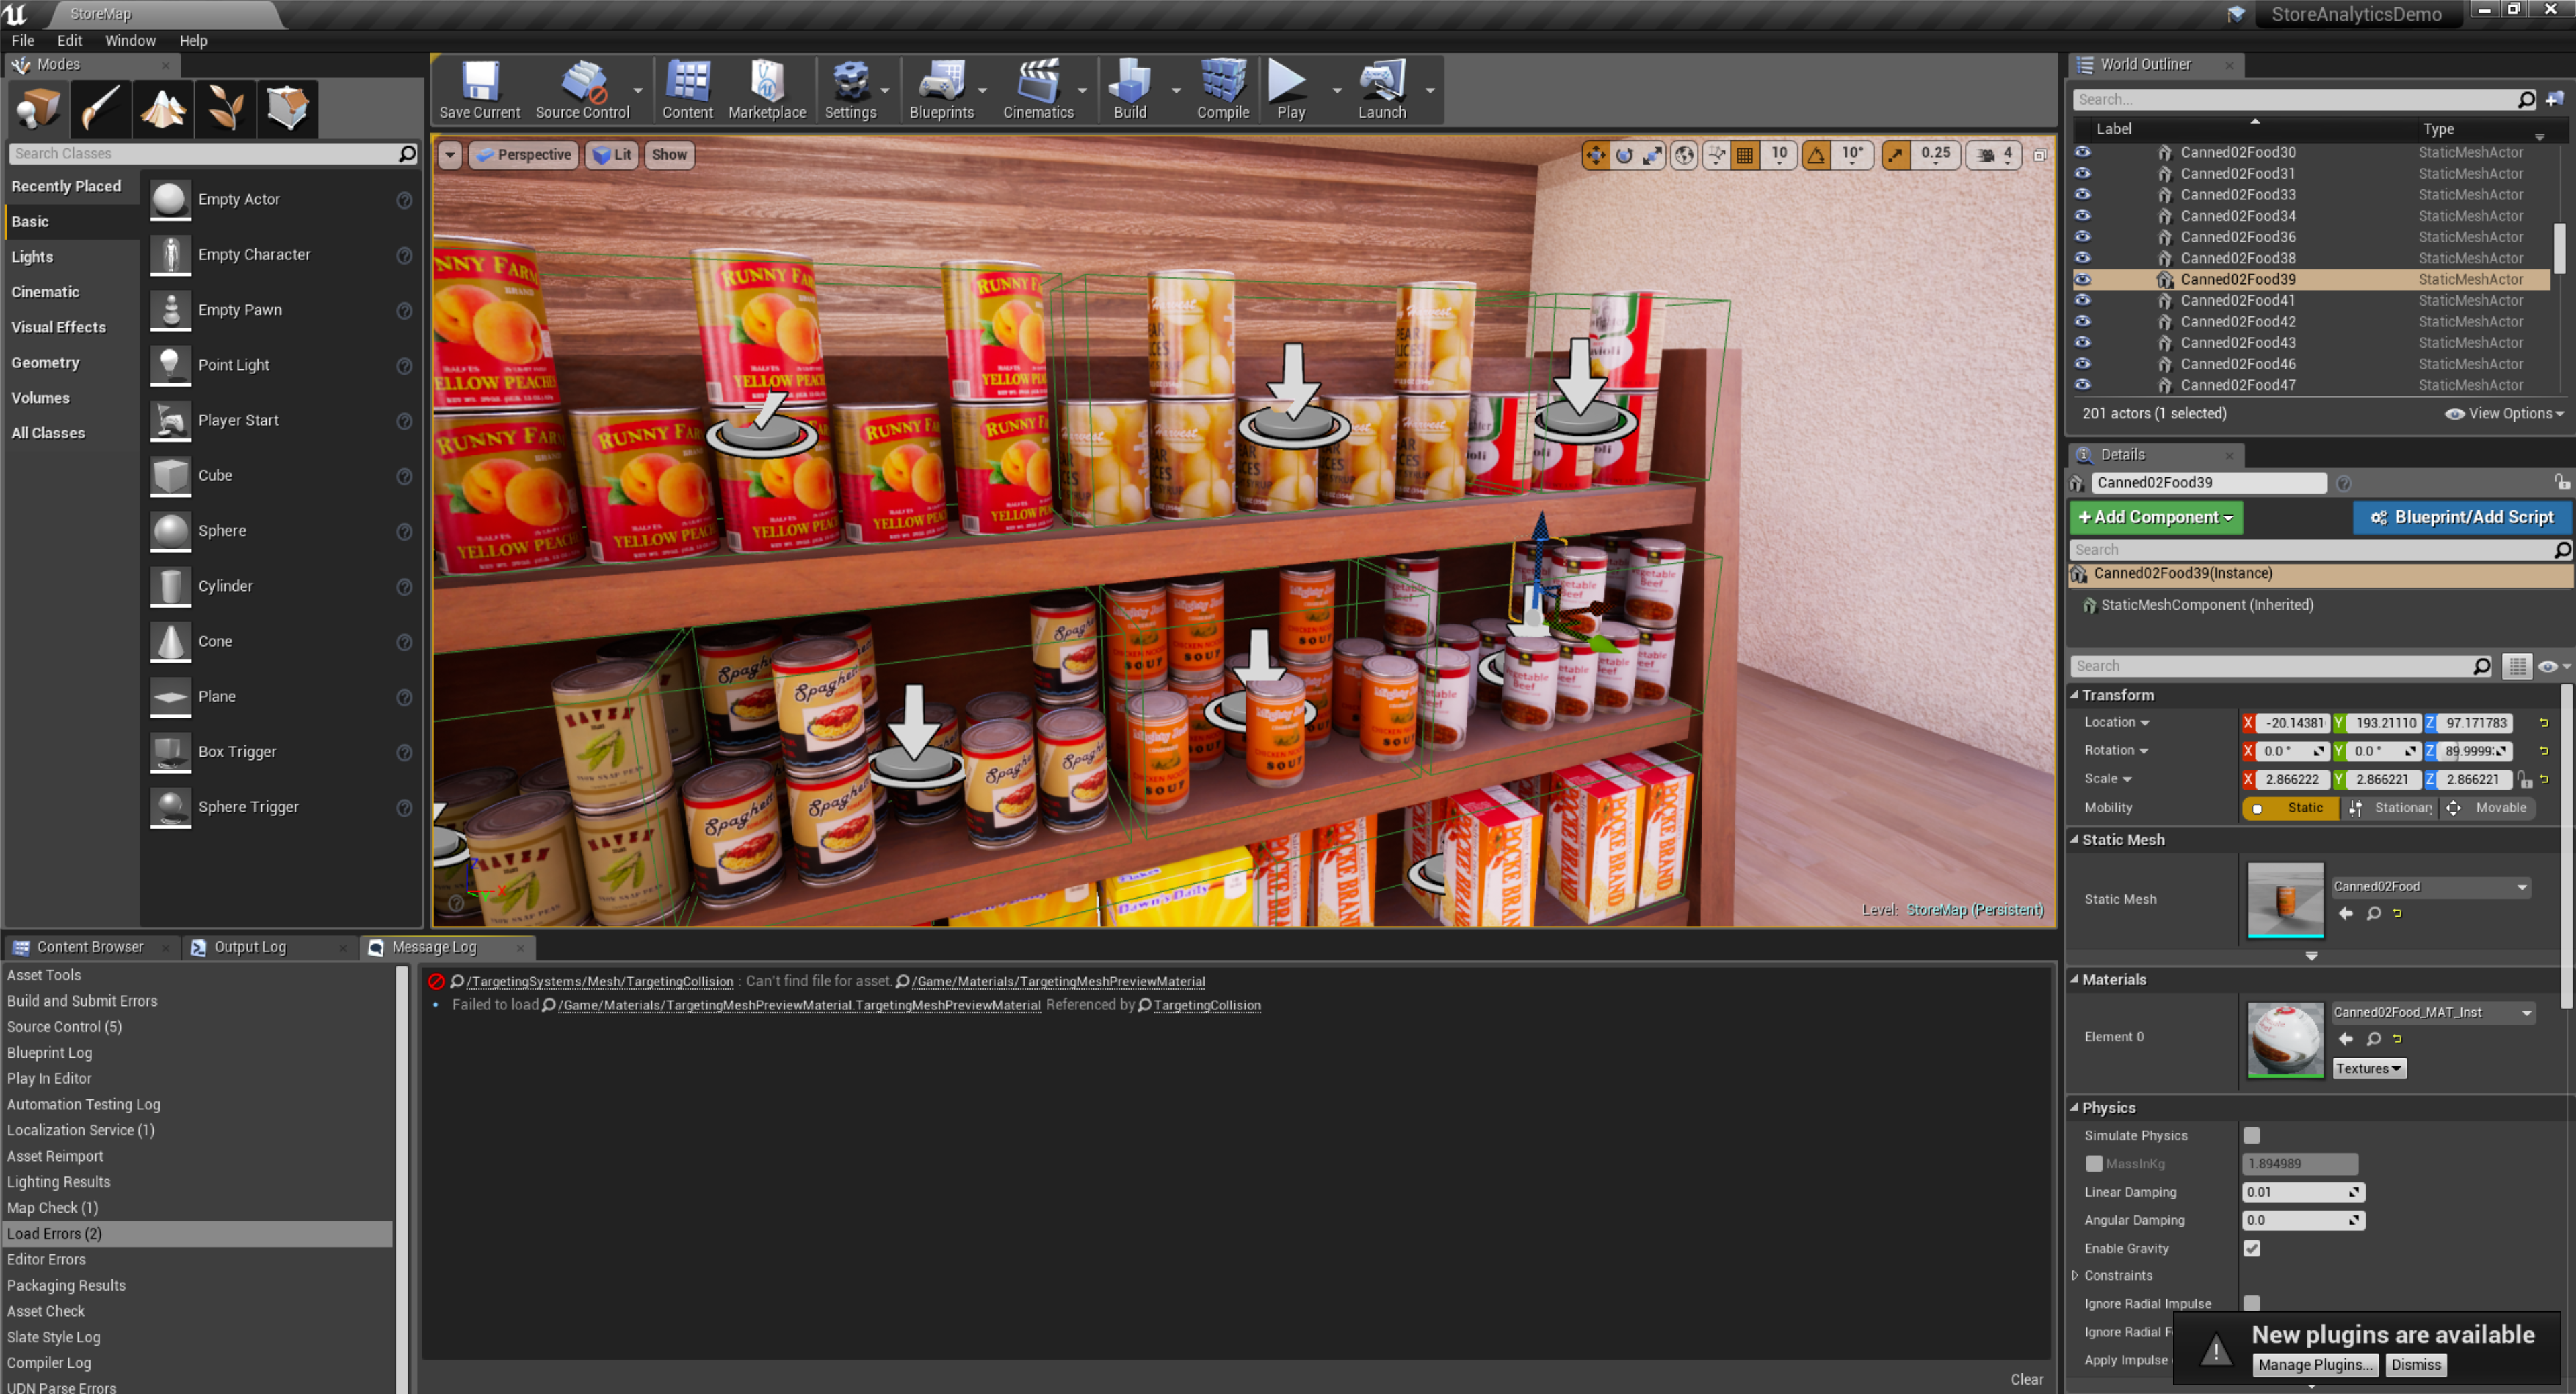
\includegraphics[width=\textwidth]{gfx/browsablestoreanalyticseditoropened.png}

Next to \texttt{Play} on the menu above the map editor there is a
dropdown arrow. Select this dropdown arrow and select
\texttt{VR\ Preview}.

\subsection{Opening A Browser to the IP
Address}\label{opening-a-browser-to-the-ip-address}

Find the Win64 machine's ip address by running \texttt{ipconfig} in a
command line console. This should return a value that includes
\texttt{192.168.XXX.XXX}. This is the local IP address. Another device
on the network may enter this IP address into its search bar to open the
dashboard. This includes anybody's phone, so you may invite people to
opepn the dashboard on their phones if you like.
